%-------------------------------------------------------
\section{Modelo Propuesto}
%-------------------------------------------------------
\subsection{Modelos Bio-inspirados / Social-inspirados}
\begin{frame}{Modelos Bio-inspirados - Distribución de Polen}{Modelo Propuesto}
%-------------------------------------------------------
    \begin{figure}				
		\fbox{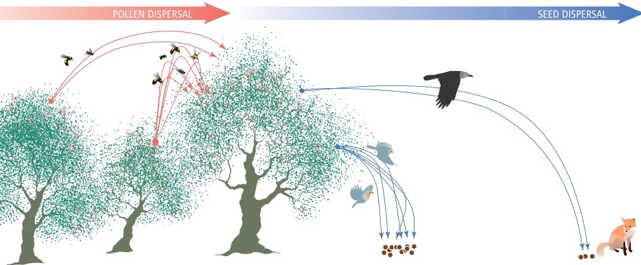
\includegraphics[width=\textwidth,keepaspectratio]{Figures/Pollen.PNG}}
		\caption{\small \sl Distribución de Polen \cite{pollen}}
		\label{figure:Pollen}
    \end{figure}
\end{frame}
%-------------------------------------------------------
%\begin{frame}{Modelos Bio-inspirados- Inteligencia de Enjambres}{Modelo Propuesto}
%-------------------------------------------------------
%    \begin{figure}				
%		\fbox{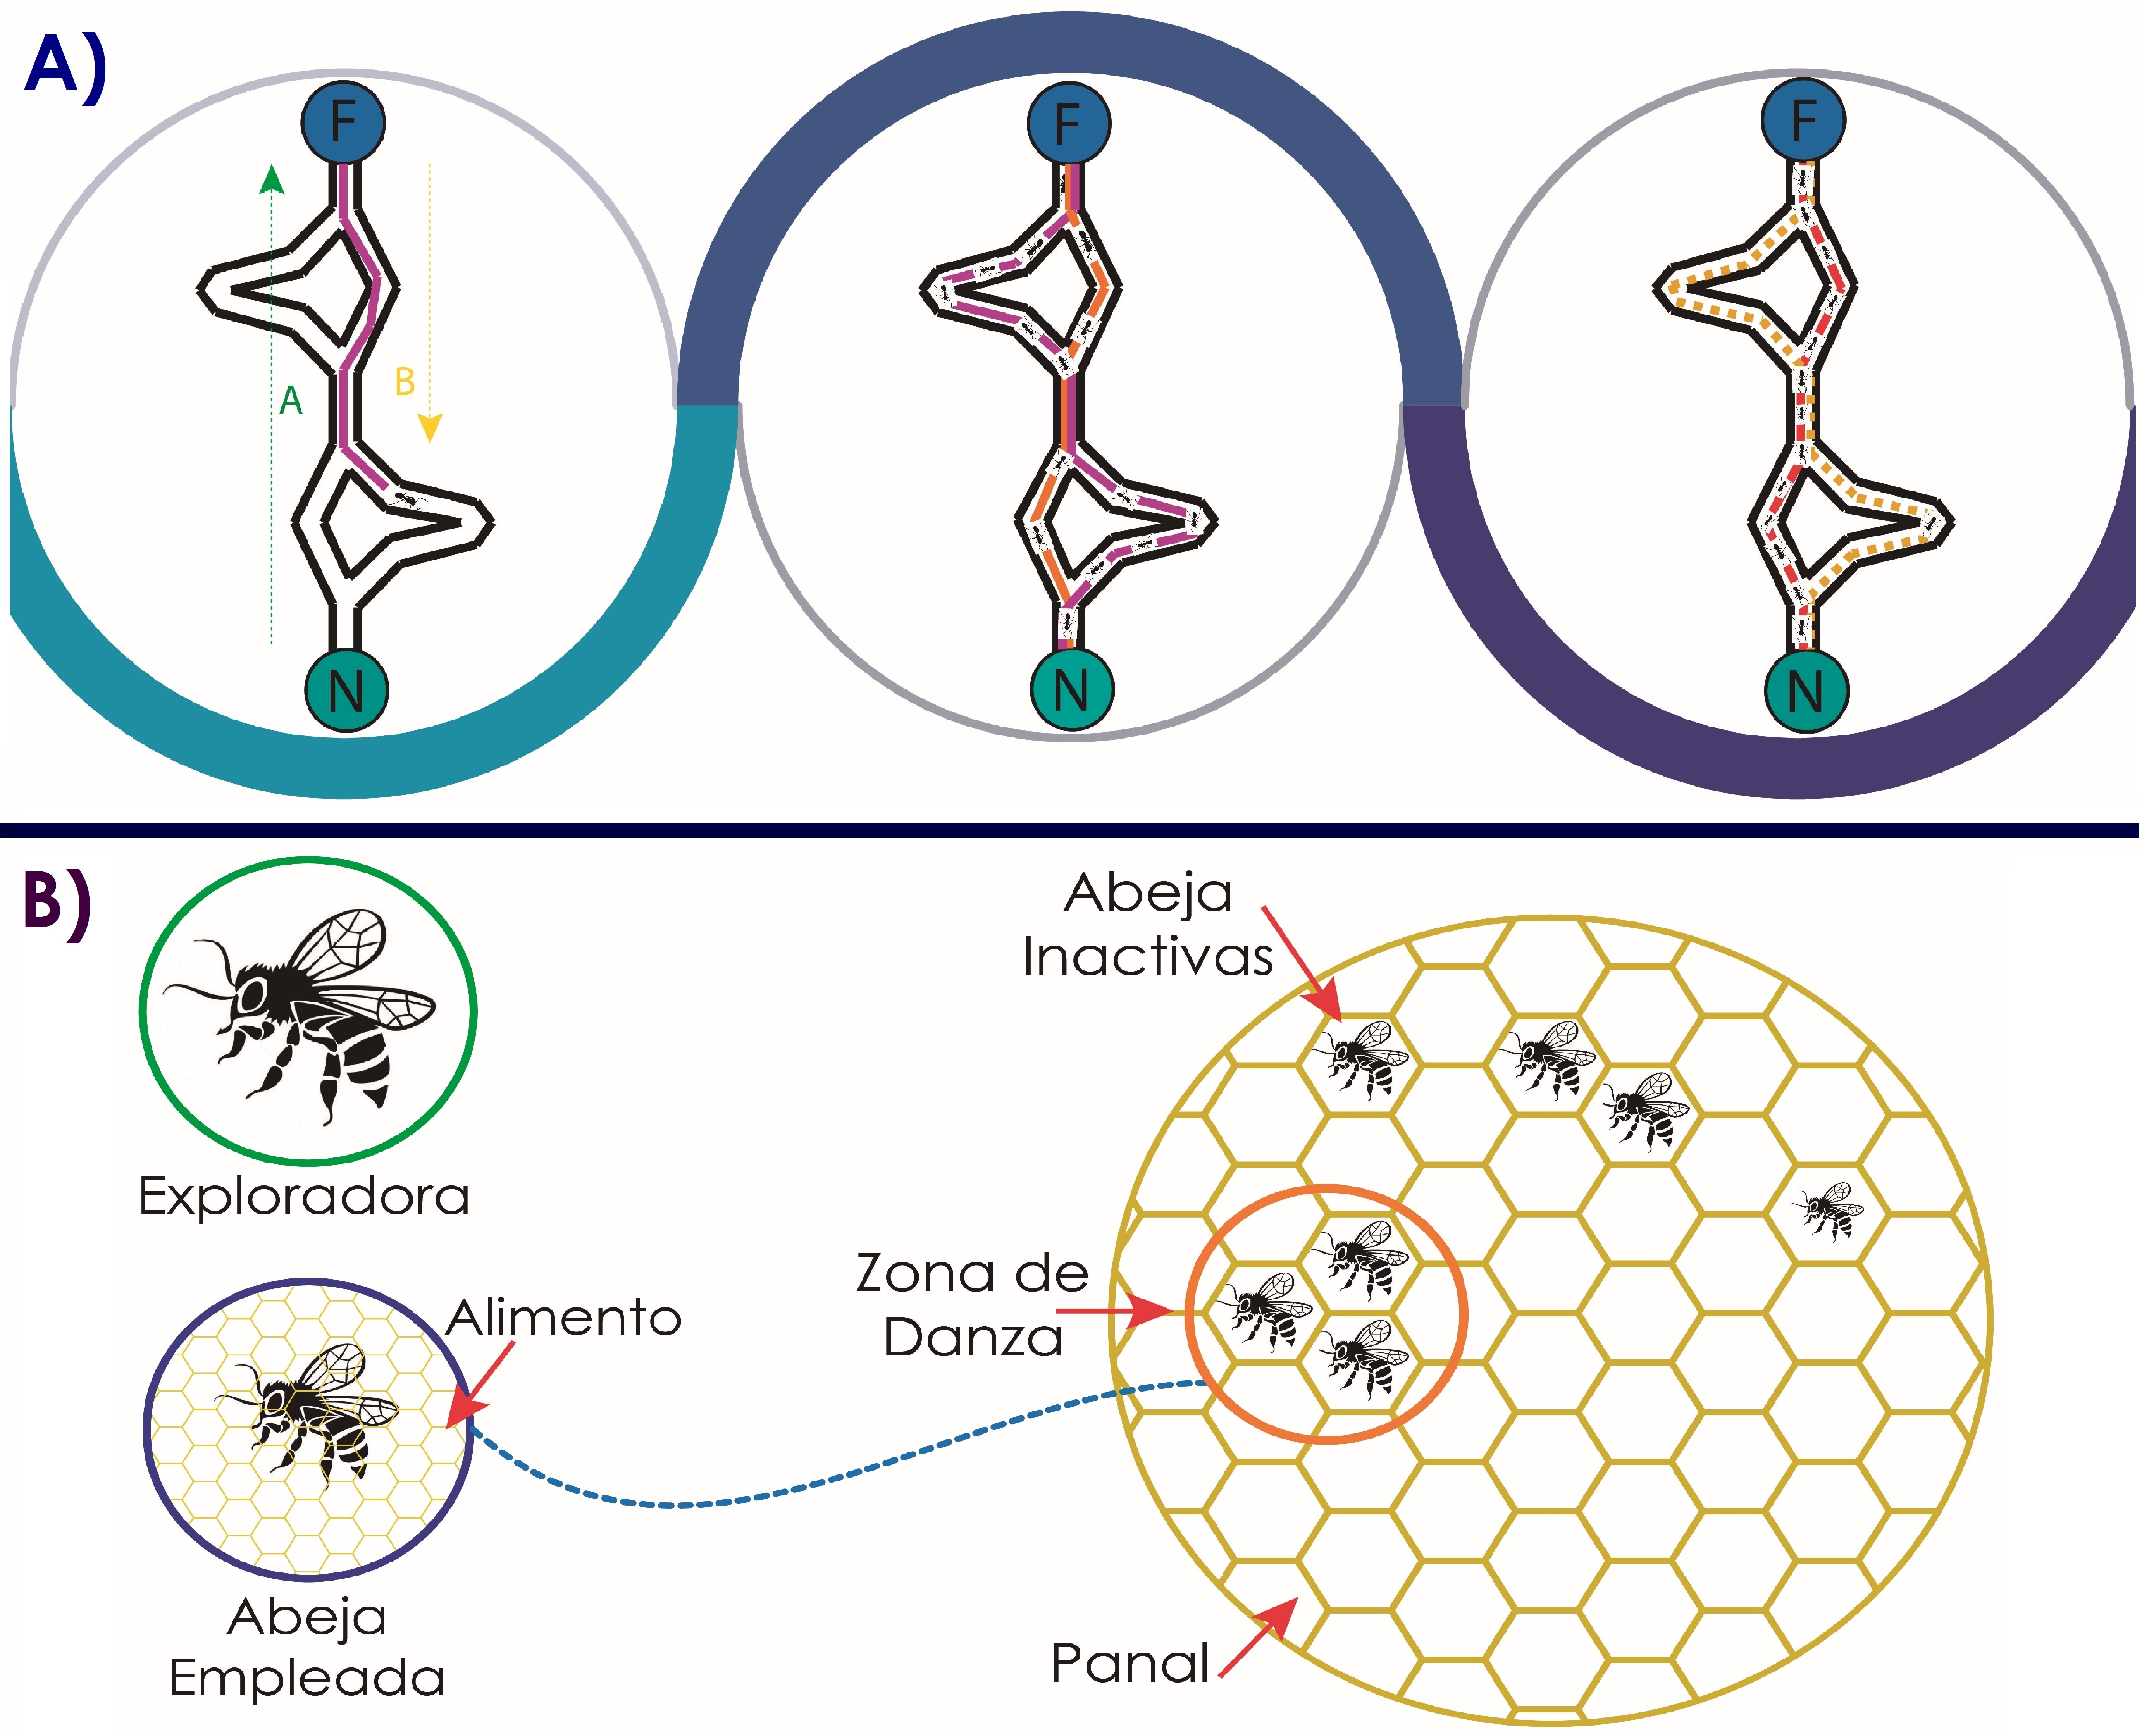
\includegraphics[height=0.7\textheight,keepaspectratio]{Figures/ants-bees.jpg}}
%		\caption{\small \sl Inteligencia de Enjambres\cite{chanPSO}}
%		\label{figure:Swarm}
%    \end{figure}
%\end{frame}
%-------------------------------------------------------
\begin{frame}{Modelos Social-inspirados- Modelo TLÖN}{Modelo Propuesto}
%-------------------------------------------------------
    \begin{figure}				
		\fbox{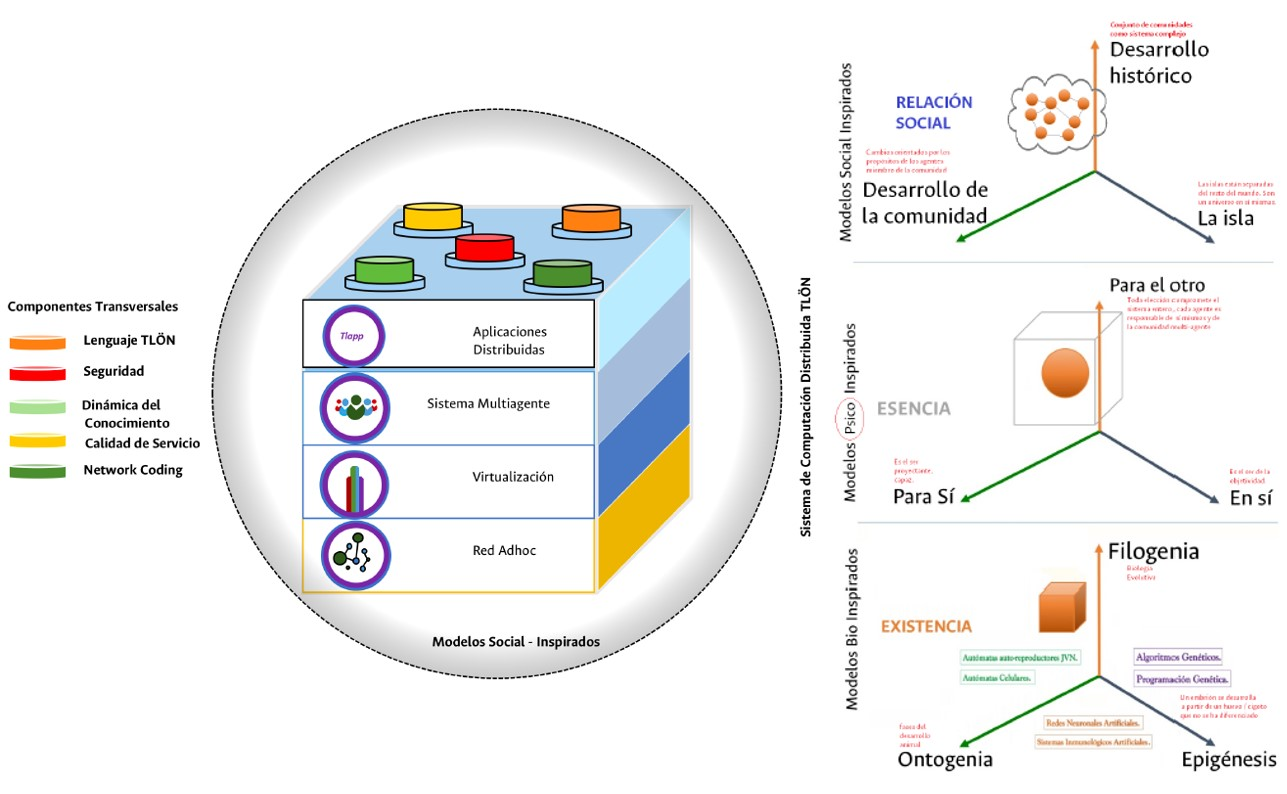
\includegraphics[height=0.55\textheight,keepaspectratio]{Sustentacion/Figures/ModeloTLON2.jpg}}
		\caption{\small \sl Modelo TLÖN [Disponible: tlon.unal.edu.co]}
		\label{figure:TLON}
    \end{figure}
\end{frame}
%-------------------------------------------------------
\subsection{Características}
\begin{frame}{Arquitectura}{Modelo propuesto}
%-------------------------------------------------------
    \begin{figure}				
		\fbox{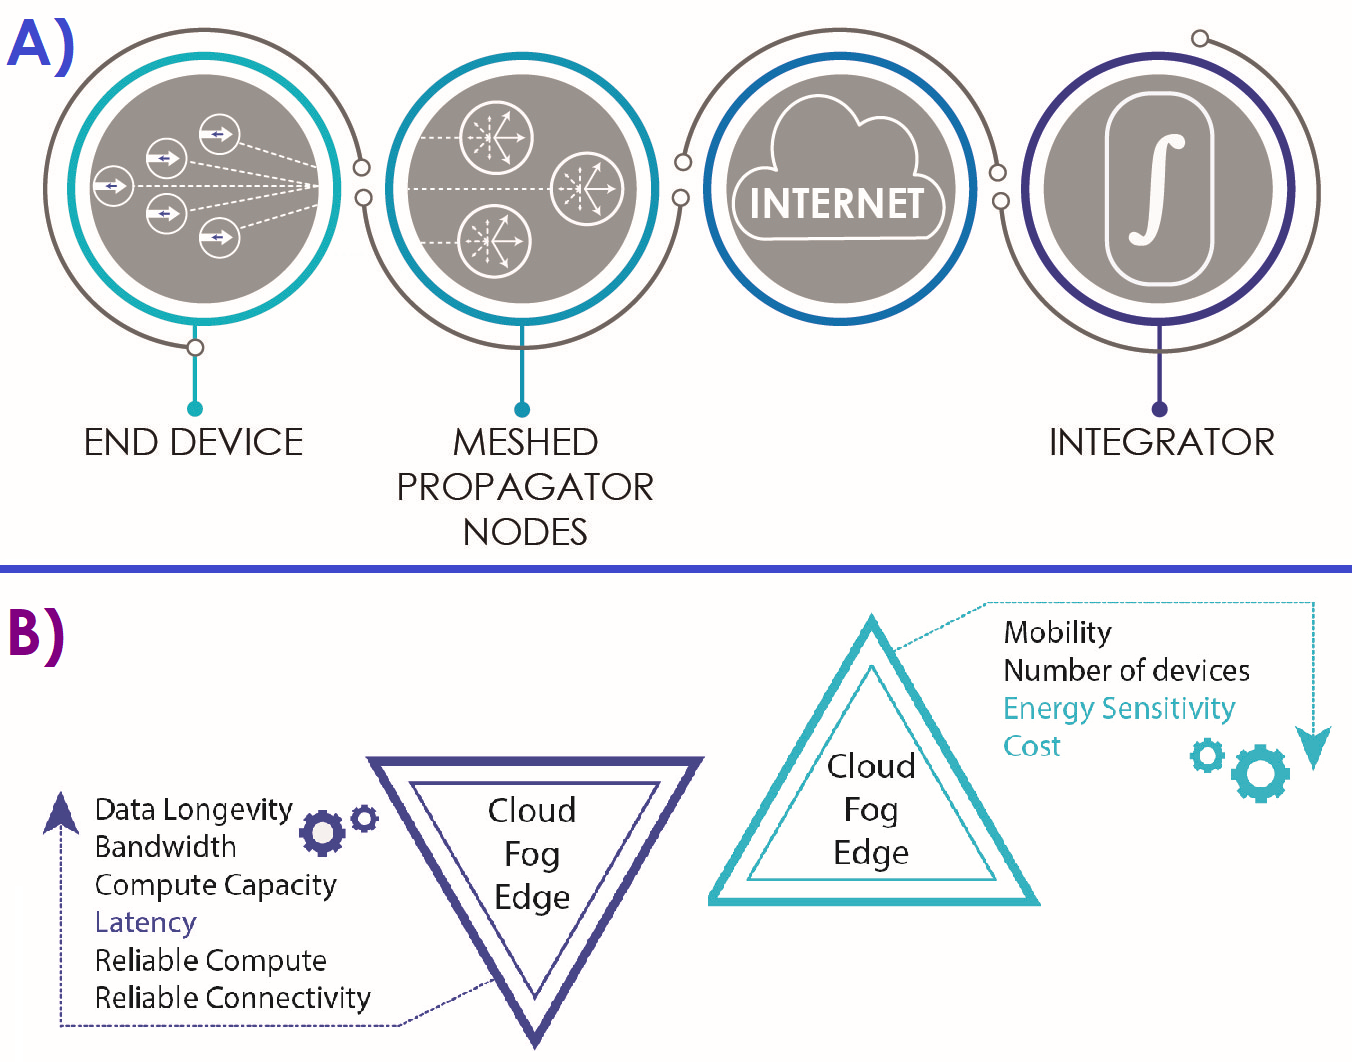
\includegraphics[height=0.68\textheight,keepaspectratio]{Sustentacion/Figures/Arquitectura.png}}
		\caption{\small \sl Arquitectura del modelo \cite{RethinkIOT,MobileEdgeComputing1,MobileEdgeComputing2,FogColony1}}
		\label{figure:Draft}
    \end{figure}
\end{frame}
%-------------------------------------------------------
\begin{frame}{Características - Datagrama e Identificadores}{Modelo propuesto}	
%-------------------------------------------------------
    \begin{figure}				
		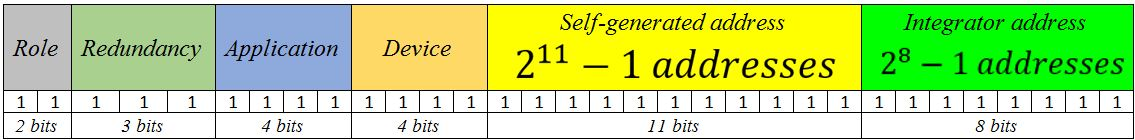
\includegraphics[width=\textwidth,height=0.7\textheight,keepaspectratio]{Figures/Datagram2.JPG}
%		\caption{\small \sl Datagram}
%		\label{figure:Datagram}
%    \end{figure}
%    \begin{figure}		
\\
		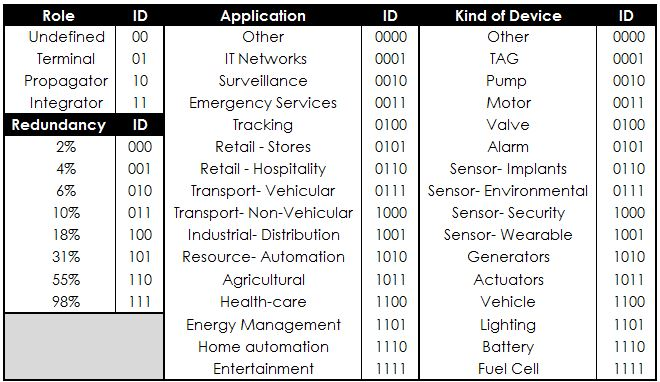
\includegraphics[width=0.85\textwidth,height=0.85\textheight,keepaspectratio]{Figures/IDs.JPG}
		\caption{\small \sl Datagrama e Identificadores externos [Fuente Propia]}
		\label{figure:Identifiers}
    \end{figure}
\end{frame}
%-------------------------------------------------------
\begin{frame}{Características - Modelo matemático}{Modelo Propuesto}	
%-------------------------------------------------------
\begin{align}
AS_{propagator} &= 2^{11+r+a+d}-1  \label{eqn1}\\
AS_{integrator} &= 2^{8+r+a+d}-1  \label{eqn2}\\
Max \# Devices &= AS_{propagator}*AS_{integrator}  \label{eqn3}\\
Min \# Propagator(n) &= \left[ \frac{\# Terminals}{AS_{propagator}} \right ] + \left[D(n)(r+a+d) \right ] \label{eqn4}
\end{align}
Donde:\\
$r$ distintos niveles de redundancia.\\
$a$ cantidad de distintas aplicaciones.\\
$d$ cantidad de distintos tipos de dispositivos.\\
$D(n)$ función de densidad de red en términos del número de nodos.\\
\end{frame}
%-------------------------------------------------------
\subsection{Máquina de Estados Finitos}
\begin{frame}{Máquina de Estados Finitos}	{Modelo Propuesto}
%-------------------------------------------------------
    \begin{figure}				
		\fbox{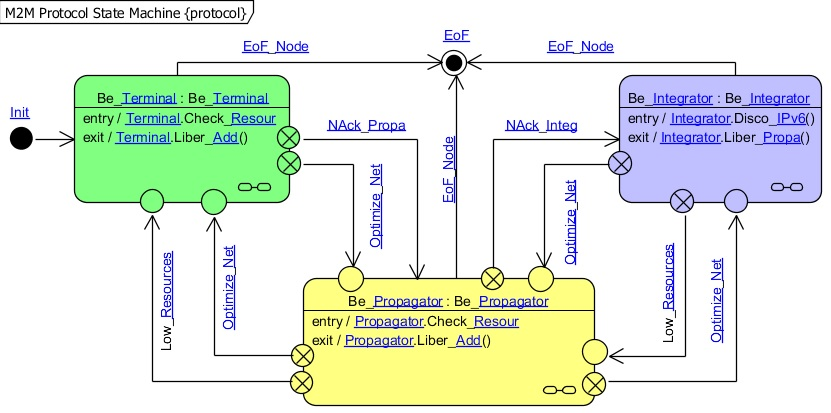
\includegraphics[width=1.0\textwidth,height=1.0\textheight,keepaspectratio]{Figures/M2M_FSM1.jpg}}
		\caption{\small \sl Protocol Finite State Machine [Fuente Propia]}
		\label{figure:ProtocolFSM}
    \end{figure}
\end{frame}
%-------------------------------------------------------
\subsection{Implementación C++}
\begin{frame}{Implementación C++}{Modelo Propuesto}
%-------------------------------------------------------
    \begin{figure}				
		\fbox{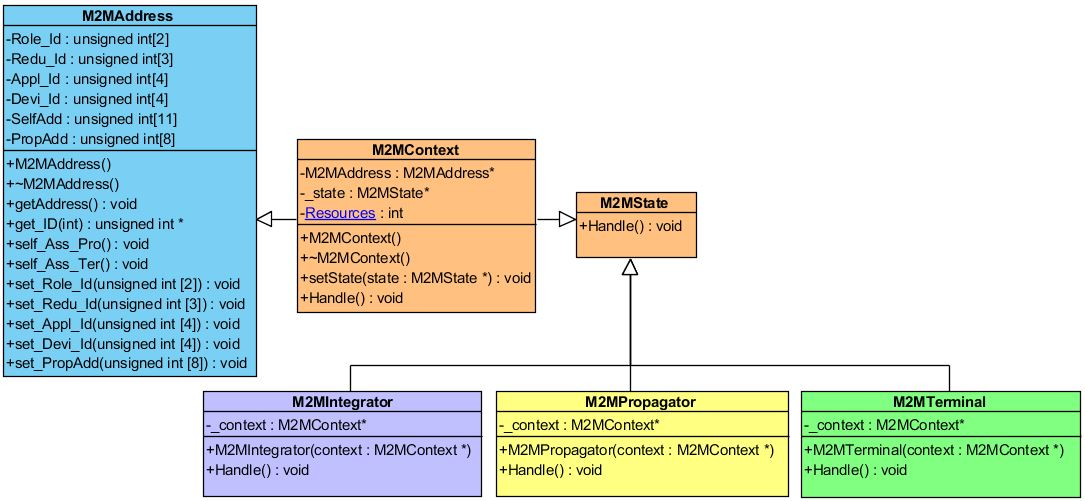
\includegraphics[width=1.05\textwidth,height=1.0\textheight,keepaspectratio]{Figures/DiagramaClases.JPG}}
		\caption{\small \sl Diagrama de Clases [Fuente Propia]}
		\label{figure:DiagramaClases}
    \end{figure}
\end{frame}
%-------------------------------------------------------
\subsection{Implementación NS-3}
\begin{frame}{Implementación NS-3}{Modelo Propuesto}	
%-------------------------------------------------------
    \begin{figure}				
		\fbox{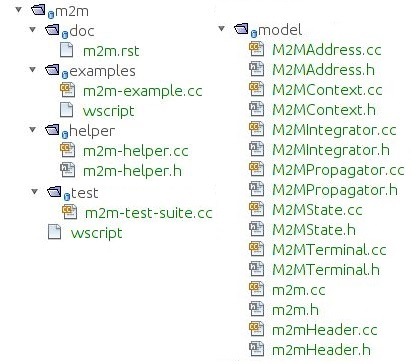
\includegraphics[width=0.6\textwidth,height=1.07\textheight,keepaspectratio]{Figures/NS3.JPG}}
		\caption{\small \sl Librería m2m: \url{https://gitlab.com/tlon-unal/m2m}\\}
		\label{figure:ImplementacionNS3}
    \end{figure}
\end{frame}
%-------------------------------------------------------